\documentclass[26pt, paperwidth=36in,paperheight=48in]{tikzposter} % See Section 3
\tikzposterlatexaffectionproofoff
\usepackage{helvet}
\renewcommand{\familydefault}{\sfdefault}
\usepackage[T1]{fontenc}
\usepackage{braket}
\usepackage{subcaption}
\usepackage{graphicx}
\usepackage{calc}
\usepackage[export]{adjustbox}


\newcommand{\myfont}{\fontsize{24}{30}\selectfont}
\newcommand{\mysmallerfont}{\fontsize{20}{30}\selectfont}

% title stuff
\makeatletter
\def\title#1{\gdef\@title{\scalebox{\TP@titletextscale}{%
			\begin{minipage}[t]{\linewidth}
				\centering
				#1
				\par
				\vspace{0.5em}
			\end{minipage}%
}}}
\makeatother


\title{
	\fontsize{76}{80} \selectfont {Hydrodynamic Properties\\ \vspace{7pt} \hspace{3pt} of the Unitary Fermi Gas}
}

\author{
	\fontsize{36}{50} \selectfont Eric Wolf, Huan Q Bui, Parth B Patel, Zhenjie Yan, Biswaroop Mukherjee, Carsten Robens, Richard Fletcher, Martin Zwierlein} 
\institute{
	\fontsize{36}{70} \selectfont MIT-Harvard Center for Ultracold Atoms, Research Laboratory of Electronics,\\\vspace{20pt}Massachusetts Institute of Technology, Cambridge, MA 02139} % See Section 4.1


\makeatletter
\renewcommand\TP@maketitle{\centering
	\begin{minipage}{0.17\linewidth}%
		\vspace{-50pt}
		
\includegraphics[width=\textwidth]{figures/header/cua-logo.pdf}
	\end{minipage}%
	\hspace{3.7cm}
	\begin{minipage}{0.55\linewidth}\centering
		\color{titlefgcolor}
		{\@title \par}
	\end{minipage}\hfill
	\begin{minipage}{0.23\linewidth}
		\vspace{-50pt}
		
\includegraphics[width=\textwidth]{figures/header/mit.eps}
	\end{minipage}%
	\vspace*{12pt}
	{\huge \@author \par}
	\vspace*{20pt}
	{\LARGE \@institute}%
}%
\makeatother

%%% end of title stuff




\usetheme{Default} % See Section 5
\usecolorpalette{Default}
\useblockstyle{Default}
%\usecolorstyle[colorPalette=BrownOrangeBlue,colorOne=blue,colorTwo=black,colorThree=green]{Britain}
\definecolor{BEC1blue}{rgb}{0, 0.14,0.5}
\definecolor{BEC1grey}{rgb}{0.89, 0.84, 0.84}
\colorlet{backgroundcolor}{BEC1blue}
\colorlet{framecolor}{white}
\colorlet{titlebgcolor}{white}
\colorlet{notefrcolor}{white} 
\colorlet{noteframecolor}{white} 
\colorlet{notebgcolor}{white}




\definebackgroundstyle{BEC1}{
	\draw[line width=0pt, 
	left color = backgroundcolor, 
	right color    = backgroundcolor!60!white] (bottomleft) rectangle (topright);
	%\draw[draw=none, line width=0pt, bottom color=titlebgcolor, top
	%color=framecolor] (bottomleft) rectangle ($(bottomleft)+(\textwidth,3)$);
}

\usebackgroundstyle{BEC1}


\usepackage{blindtext}
\usepackage{comment}






\begin{document}
	
\maketitle[width=0.96\textwidth] % See Section 4.1


%% first row
\begin{columns} % See Section 4.4
\column{0.4}
\colorlet{blocktitlebgcolor}{BEC1grey}
\block[]{\textcolor{BEC1blue}{Unitary Fermi Gas in a Box Potential}}
{



\begin{minipage}{0.17\textwidth}
	\flushleft
	\vspace{0.5cm}
	\textbf{Unitary Fermi Gas}
	\vspace{0.5cm}
	\myfont
	\begin{itemize}
		%\item Strongly-interacting fermion systems - difficult to analyze a priori
		
		\item Relevant to systems ranging from neutron stars to high-${T_c}$ superconductors
		
		\item Unitary Fermi gas is scale-invariant
		
		\item Realize unitarity with $\ket{1} - \ket{3}$ Feshbach resonance in $^6$Li
		
		\item Evaporatively cool spin mixture to below $T_F$
	\end{itemize}
\vspace{2cm}
\end{minipage}
\hspace{0.6cm}
\begin{minipage}{0.15\textwidth}
	\begin{minipage}{\textwidth}
		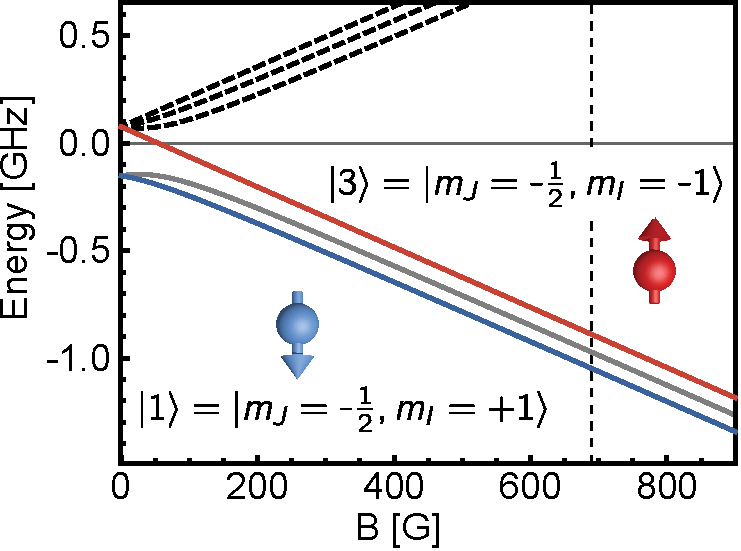
\includegraphics[width=1\textwidth]{figures/BreitRabiLi6.pdf}
	\end{minipage}
	
	\vspace{0.5cm}
	\hspace{-2cm}
	\begin{minipage}{\textwidth}
		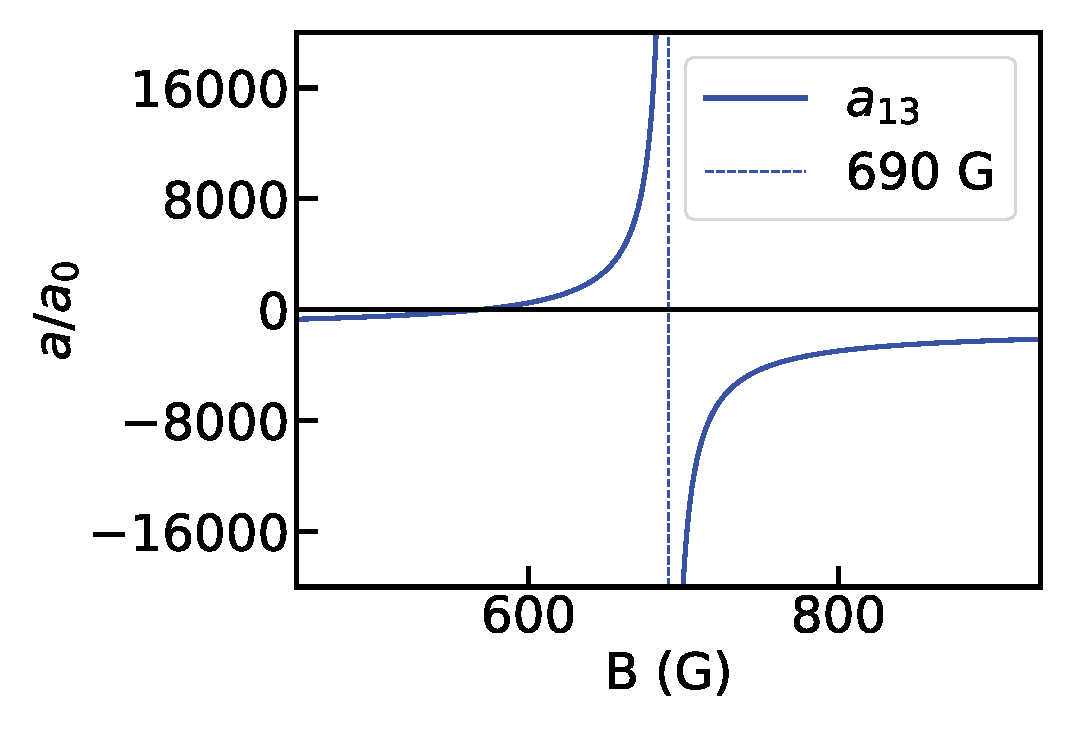
\includegraphics[width=1.15\textwidth]{figures/Feshbach_Plot_Redone.eps}
	\end{minipage}
	
	
\end{minipage}


%%%%

\vspace{-0.0cm}
\begin{minipage}{0.14\textwidth}
	\flushleft
	\textbf{Box Potential [1]}
	\vspace{0.5cm}
	\myfont
	\begin{itemize}
		\item Hollow blue-detuned beams realize (quasi) flat potential
		
		\item Reduces influence of trap averaging \& targets smaller range of densities
		
		\item Momentum imaging possible via residual axial harmonic trap
		
		%\item Residual harmonic trap in axial dimension allows momentum-space imaging
	\end{itemize}
\end{minipage}
\hspace{0.2cm}
\begin{minipage}{0.15\textwidth}
	\centering
	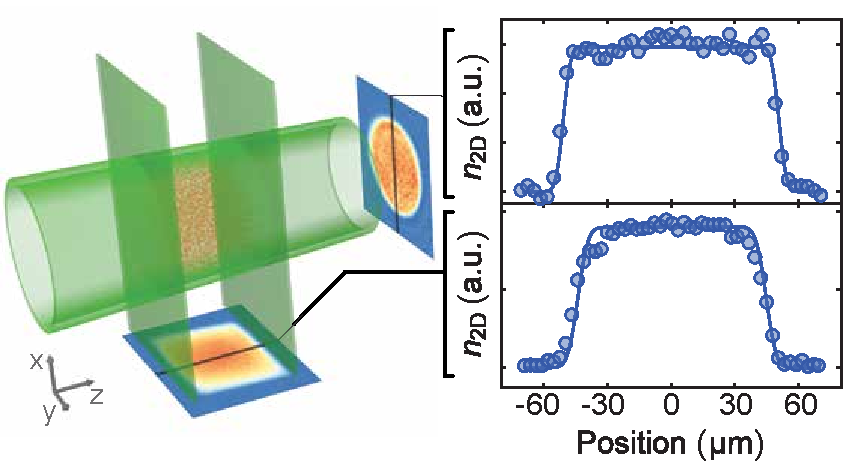
\includegraphics[scale=1.2]{figures/box_cartoon.pdf}
\end{minipage}

\centering
\vspace{0.53cm}
\begin{minipage}{0.3\textwidth}
	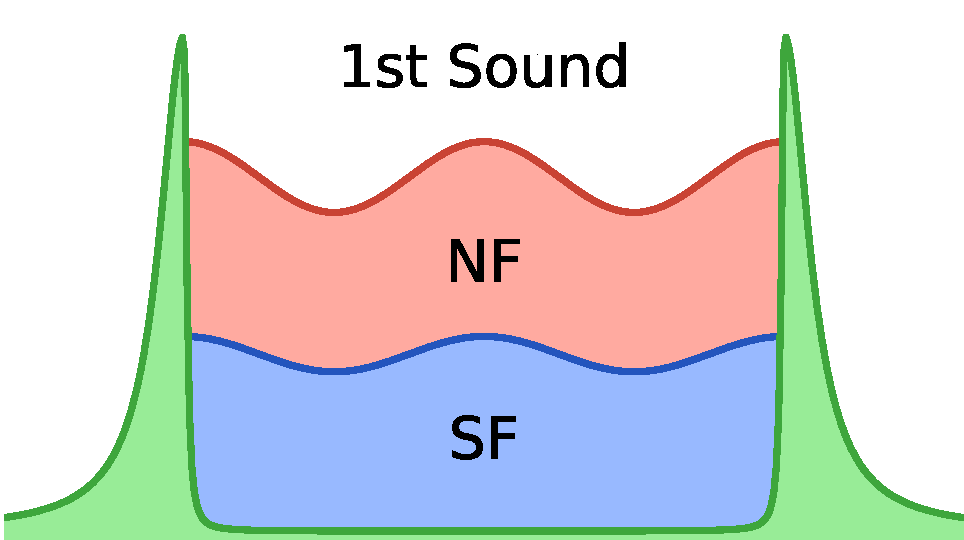
\includegraphics[width=0.49\textwidth]{figures/first_sound_cartoon.pdf}
	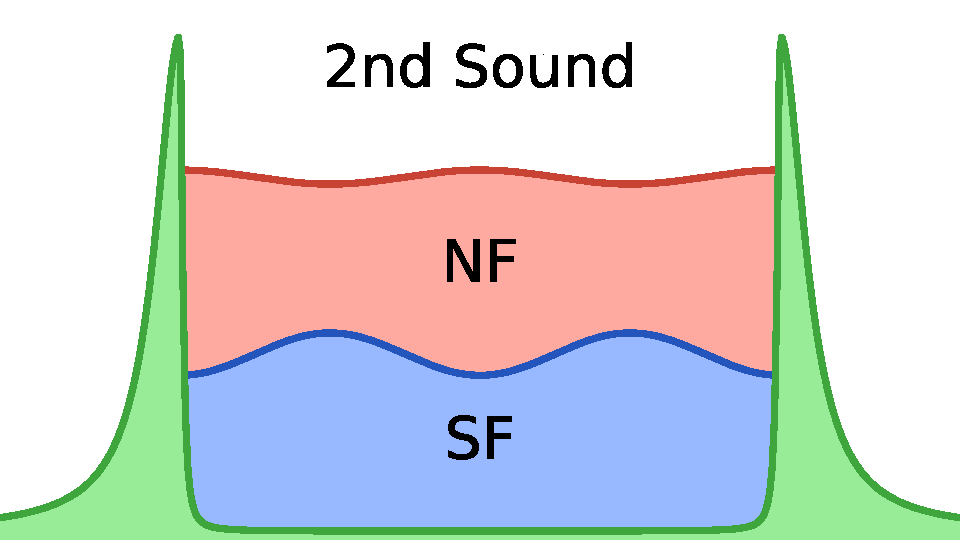
\includegraphics[width=0.49\textwidth]{figures/second_sound_cartoon.pdf}
	%\centering{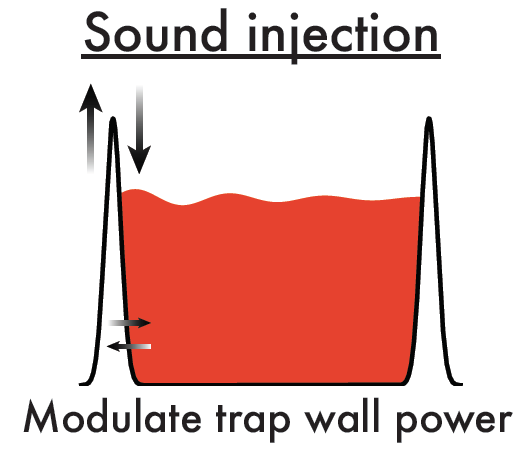
\includegraphics[width=0.49\textwidth,
	%	trim=0.6cm 1.0cm 0.6cm 0cm,clip]{figures/first_sound_injection.png}}
\end{minipage}
\vspace{0.55cm}
} 







%%%%%% 

\column{0.6}
\colorlet{blocktitlebgcolor}{BEC1grey}
\block[]{\textcolor{BEC1blue}{Density Response -- First Sound [2]}}
{
	\begin{minipage}{0.2\textwidth}
		\flushleft
		\vspace{0.5cm}
		\textbf{First Sound}
		\vspace{0.5cm}
		\myfont
		\begin{itemize}
			\item Density oscillations: in-phase oscillation of normal and superfluid phase
			
			\item Excite by shaking box walls
			
			\item Image density waves in-situ -- extract wavevector $k$ for a given $\omega$ to get $c$
			
			\item Speed of sound in scale-invariant system given by system energy $$mc^2 = \frac{10}{9} \frac{E}{N}$$
		\end{itemize}
		
		%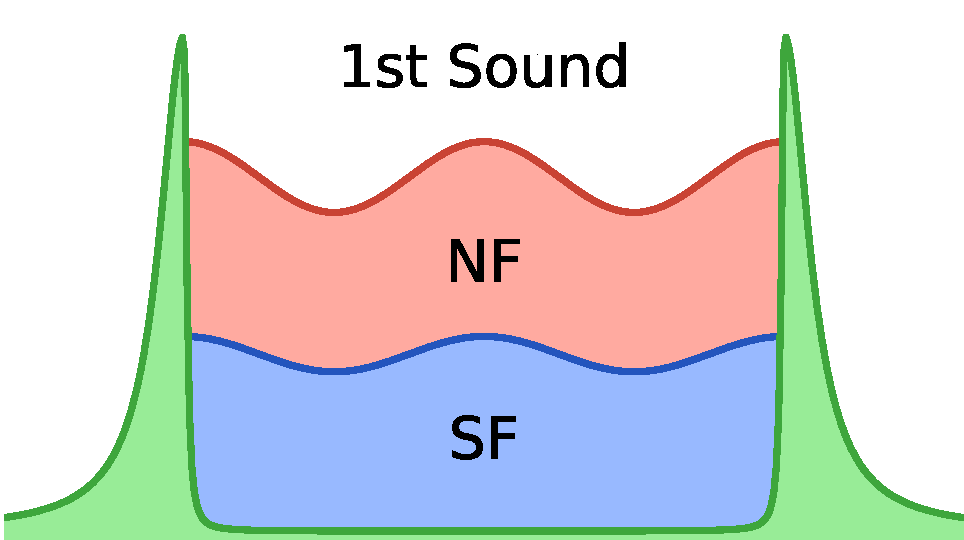
\includegraphics[width=0.49\textwidth]{figures/first_sound_cartoon.pdf}
		\centering{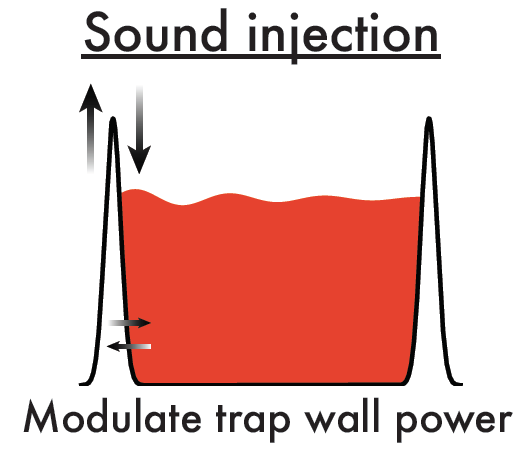
\includegraphics[width=0.45\textwidth,
		trim=0.6cm 1.0cm 0.6cm 0cm,clip]{figures/first_sound_injection.png}}
	\end{minipage}
	\hspace{0.25cm}
	\begin{minipage}{0.3\textwidth}
		\centering
		\raisebox{-0.42\height}{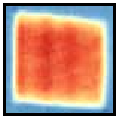
\includegraphics[width=0.26\textwidth]{figures/first_sound_shake.pdf}}
		\huge{-}
		\raisebox{-0.42\height}{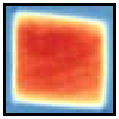
\includegraphics[width=0.26\textwidth]{figures/first_sound_background.pdf}}
		\huge{=}
		\raisebox{-0.42\height}{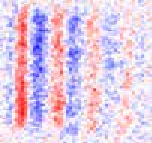
\includegraphics[width=0.26\textwidth]{figures/shake-minus-background.pdf}}\\
		
		\vspace{1.5cm}
		\hspace{-2cm}
		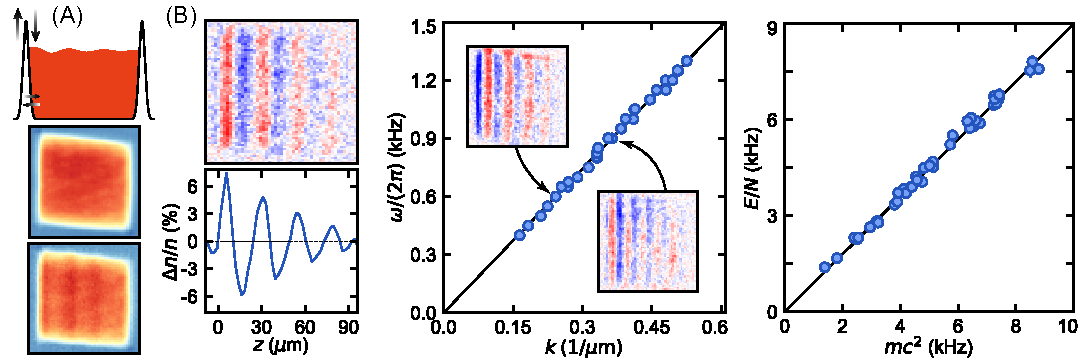
\includegraphics[width=1.1\textwidth,
		trim=6.5cm 0cm 0cm 0cm,clip]{figures/sound_diff_disp_redone.pdf}
		
	\end{minipage}
	
	\vspace{0cm}
	\begin{minipage}{0.2\textwidth}
		\flushleft
		\textbf{Resonant Modes and Dissipation}
		\vspace{0.5cm}
		\myfont
		\begin{minipage}{0.8\textwidth}
			\flushleft
			\vspace{1.2cm}
			\begin{itemize}
				\item Sound speed constrained by scale invariance, but dissipation is not
				
				\item Hydrodynamics predicts damping rate $\Gamma \propto k^2$, with proportionality constant $D_s$, the sound diffusivity
				
				\item $D_s$ depends on shear viscosity and thermal conductivity 
				
				\item Measure damping vs. $k$ using width of resonant box modes -- extract $D_s$
			\end{itemize}
		\end{minipage}
		
	\end{minipage}
	\hspace{-3cm}
	\begin{minipage}{0.13\textwidth}
		\vspace{1.7cm}
		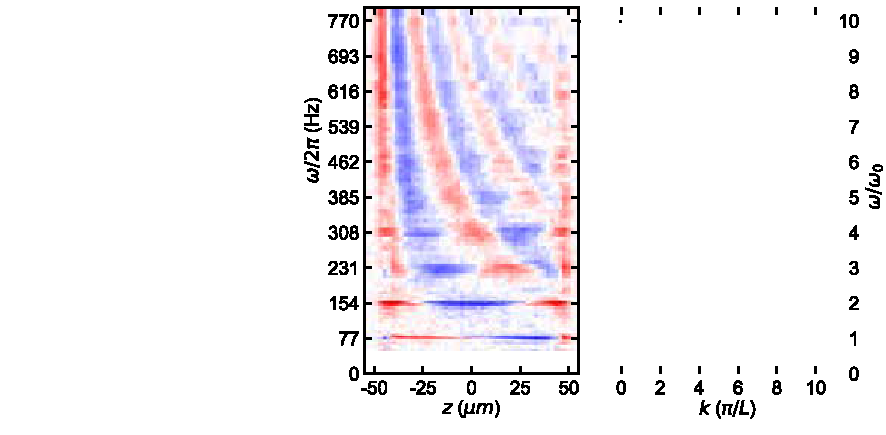
\includegraphics[width=9cm,
		trim=5cm 0cm 5.2cm 0cm,clip]{figures/fundamental_modes_redone.pdf}
	\end{minipage}
	\hspace{-2cm}
	\begin{minipage}{0.3\textwidth}
		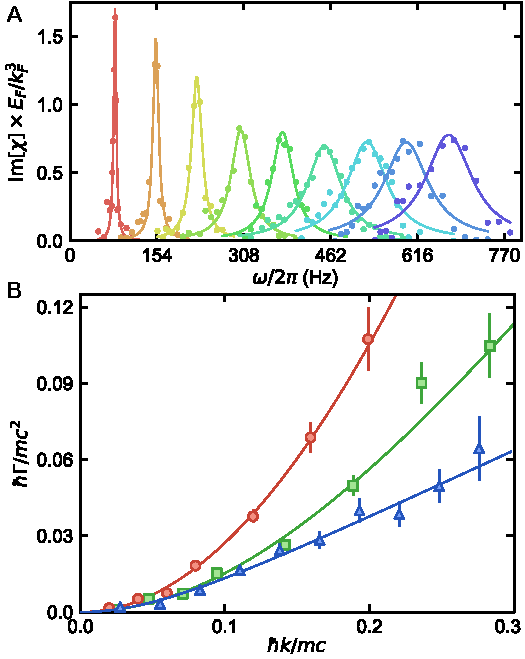
\includegraphics[width=10cm]{figures/First Sound Resonance Widths.pdf}
		\hspace{0.1cm}
		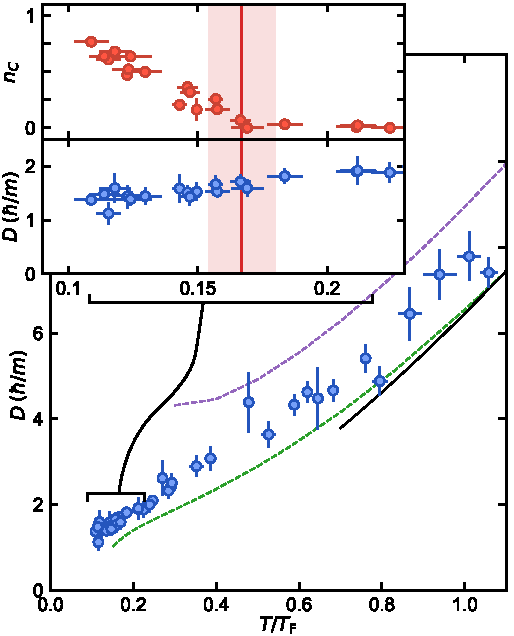
\includegraphics[width=11cm]{figures/sound_diffusivity.pdf}
	\end{minipage}
	\vspace{0.5cm}
	
	
}
%\note[targetoffsetx=9.5cm, targetoffsety=12cm, angle=0, radius=0cm,
%width=1.1cm, rotate=0, connection, linewidth=0cm,
%roundedcorners=0, innersep=0cm]{}

%\note[targetoffsetx=-3cm, targetoffsety=12cm, angle=0, radius=0cm,
%width=1.1cm, rotate=0, connection, linewidth=0cm,
%roundedcorners=0, innersep=0cm]{}
	
	
	


\end{columns}



%% second row

\begin{columns} 
	
	%%%
	
	
	%%%%%%%%%%%%%%%%%%%%%%%%%%%%%%%%%%%%%%%%%%%%%
	
	\column{0.55} 
	\colorlet{blocktitlebgcolor}{BEC1grey}
	\block[]{\textcolor{BEC1blue}{Temperature Response -- Second Sound [3]}}
	{
		\begin{minipage}{0.21\textwidth}
			\flushleft
			\vspace{0.5cm}
			\textbf{Second Sound}
			\vspace{0.5cm}
			\myfont
			\begin{itemize}
				\item Temperature oscillations: out-of-phase oscillations of normal and superfluid phase
				
				
				\item Excite oscillations by imprinting high-frequency sound waves to locally heat the gas
				
				
				\item Measure temperature locally using RF spectroscopy
				
				
				\item Second sound arises at temperatures below the superfluid transition temperature 
				
				
				\item Damping rate of second sound gives thermal conductivity
			\end{itemize}
		\end{minipage}
		\hspace{1cm}
		\begin{minipage}{0.15\textwidth}
			\vspace{-0.21cm}
			\centering
			\hspace{0.5cm}
			%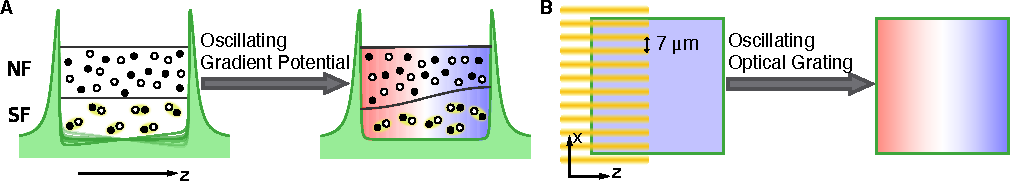
\includegraphics[width=1.7\textwidth,
			%trim=9.4cm 0cm 0cm 0cm,clip]{figures/SecondSoundExcitation.pdf}
			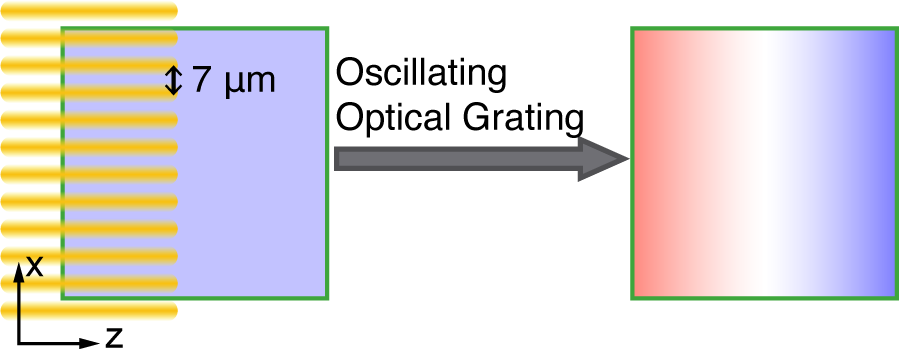
\includegraphics[width=1.7\textwidth]{figures/SecondSoundExcitationRedone.png}
			\centering
			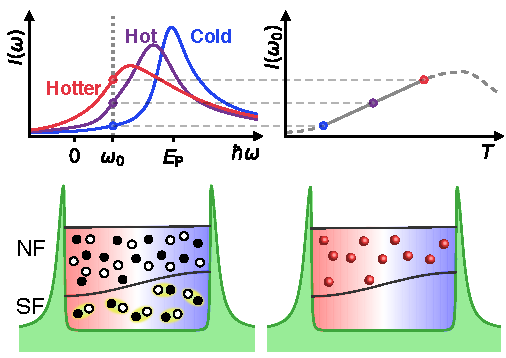
\includegraphics[width=1.7\textwidth,
			trim=0cm 3.2cm 0cm 0cm,clip]{figures/local_thermometer_redone.pdf}
		\end{minipage}
		
		
		
		%%%% 
		\vspace{0cm}
		\begin{minipage}{0.15\textwidth}
			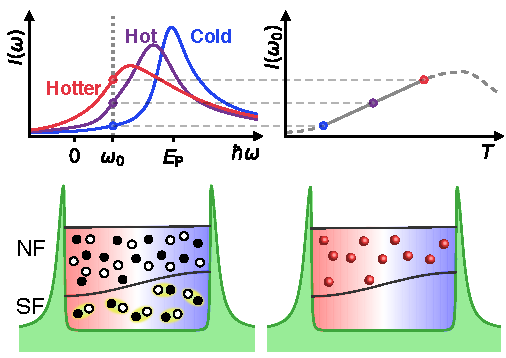
\includegraphics[width=10cm,
			trim=0cm 0cm 4.4cm 3.2cm,clip]{figures/local_thermometer_redone.pdf}\\
			
			\hspace{0.5cm}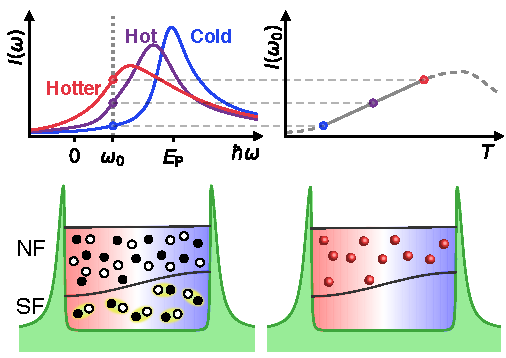
\includegraphics[width=10cm,
			trim=4.4cm 0cm 0cm 3.2cm,clip]{figures/local_thermometer_redone.pdf}
		\end{minipage}
		\hspace{-3.5cm}
		\begin{minipage}{0.2\textwidth}
			\vspace{-2cm}
			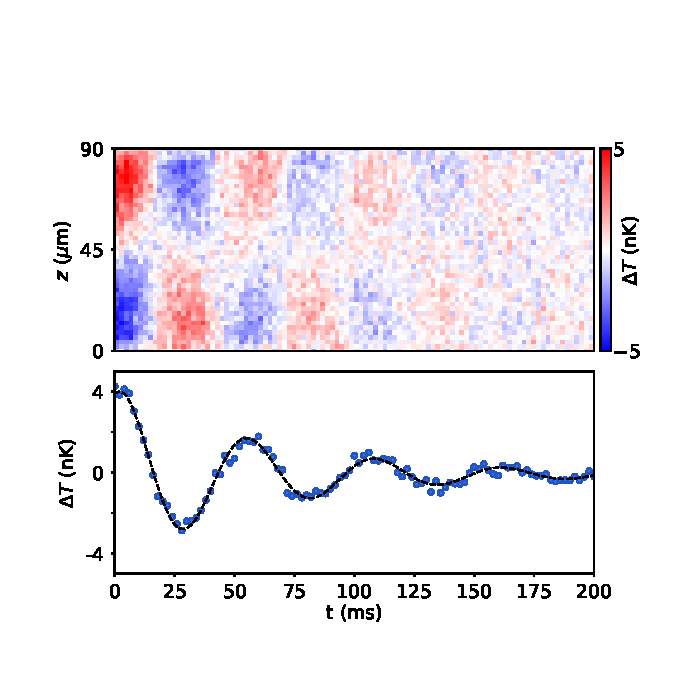
\includegraphics[width=17cm,
			trim=0cm 5.2cm 0cm 0cm,clip]{figures/TimeEvolution_Slides_noedge.pdf}\\
			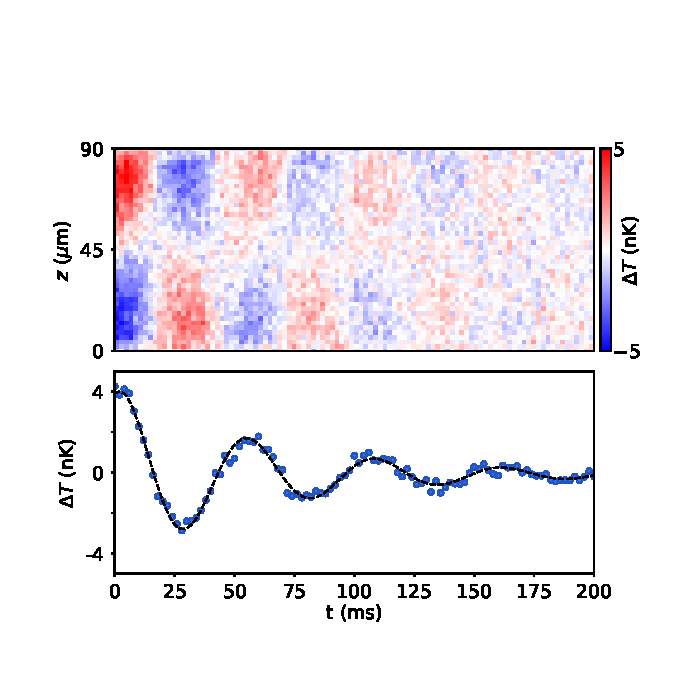
\includegraphics[width=17cm,
			trim=0cm 0cm 0cm 9.67cm,clip]{figures/TimeEvolution_Slides_noedge.pdf}\\
			
			\centering
			\vspace{-1.5cm}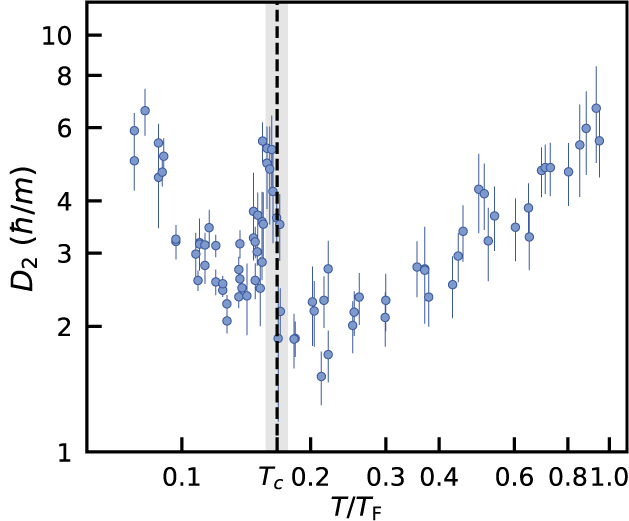
\includegraphics[width=11cm]{figures/thermal_diffusivity.png}
		\end{minipage}
		\hspace{-0.5cm}
		\begin{minipage}{0.15\textwidth}
			\vspace{2cm}
			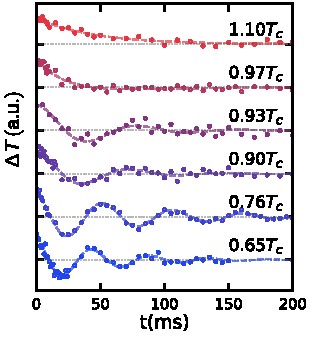
\includegraphics[width=15.5cm]{figures/LocalHeater_Waterfall 6.pdf}
		\end{minipage}
		\vspace{1cm}
	}
	
	
	%\note[targetoffsetx=-13cm, targetoffsety=0.8cm, angle=0, radius=0cm,
	%width=1.6cm, rotate=0, connection, linewidth=0cm,
	%roundedcorners=0, innersep=0cm]{}
	
	%\note[targetoffsetx=-21.6cm, targetoffsety=-8cm, angle=0, radius=0cm,
	%width=1.7cm, rotate=0, connection, linewidth=0cm,
	%roundedcorners=0, innersep=0cm]{}
	
	
	\note[targetoffsetx=-15cm, targetoffsety=-6.8cm, angle=0, radius=0cm,
	width=0.1cm, rotate=-90, connection, linewidth=0cm,
	roundedcorners=0, innersep=0cm]{
		\includegraphics[width=2.5cm]{figures/Spin_Flip_Picture_3.eps}
		
		
		
	}


	
	
	
	

	
	\column{0.45} % See Section 4.4
	\colorlet{blocktitlebgcolor}{BEC1grey}
	\block[]{\textcolor{BEC1blue}{Hydrodynamics -- Transport Properties}}
	{
		\begin{minipage}{0.38\textwidth}
			\flushleft
			%\vspace{0.5cm}
			\textbf{Hydrodynamic Quantities}
			\vspace{0.5cm}
			\myfont
			\begin{itemize}
				\item Hydrodynamic quantities above $T_c$: shear viscosity $\eta$ and thermal conductivity $\kappa$
				
				\item Bulk viscosity vanishes for scale-invariant systems; below $T_c$, superfluidity density is conserved 
				
				\item First sound dissipation given by $\kappa$ and $\eta$; second sound dissipation by $\kappa$ and $c_P$
				
				\item Together with equation of state [4], first and second sound give $\eta$ and $\kappa$ above $T_c$
			\end{itemize}
		\end{minipage}
		
		\vspace{-1cm}
		\begin{minipage}{0.48\textwidth}
			\centering
			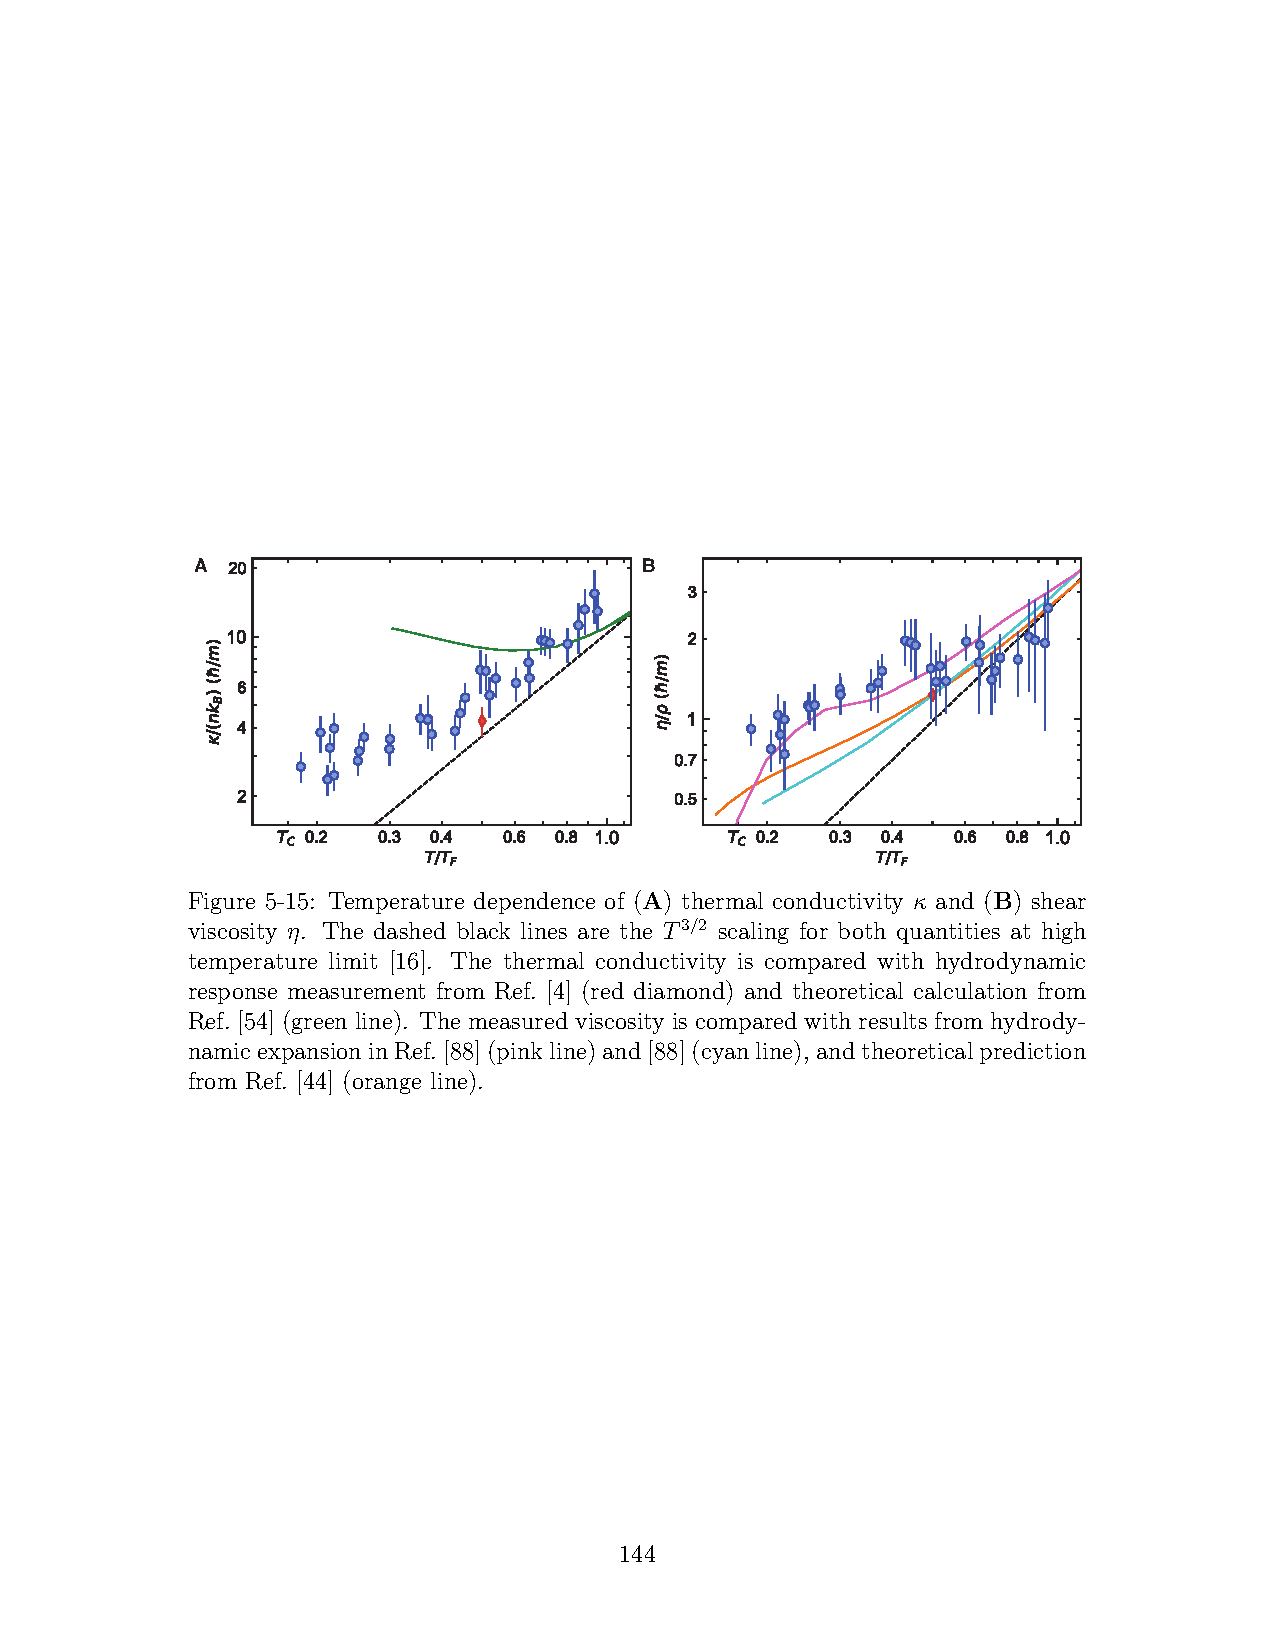
\includegraphics[width=\textwidth,
			trim=3.2cm 13cm 0cm 8.5cm,clip]{figures/transport.pdf}
		\end{minipage}
	
	
	
	\vspace{-2cm}
	\begin{minipage}{0.16\textwidth}
		\flushleft
		\textbf{Results}
		\vspace{0.5cm}
		\myfont
		\begin{itemize}
			\item Viscosity agrees with prior results and theory
			
			\item Thermal conductivity differs strongly from theory predictions near $T_c$
			
			\item Prandtl number $\frac{c_P \eta}{\kappa}$, ratio of momentum to thermal diffusivity, remains close to typical $2/3$ value for gases 
		\end{itemize}
		
	\end{minipage}
	\hspace{1cm}
	\begin{minipage}{0.22\textwidth}
		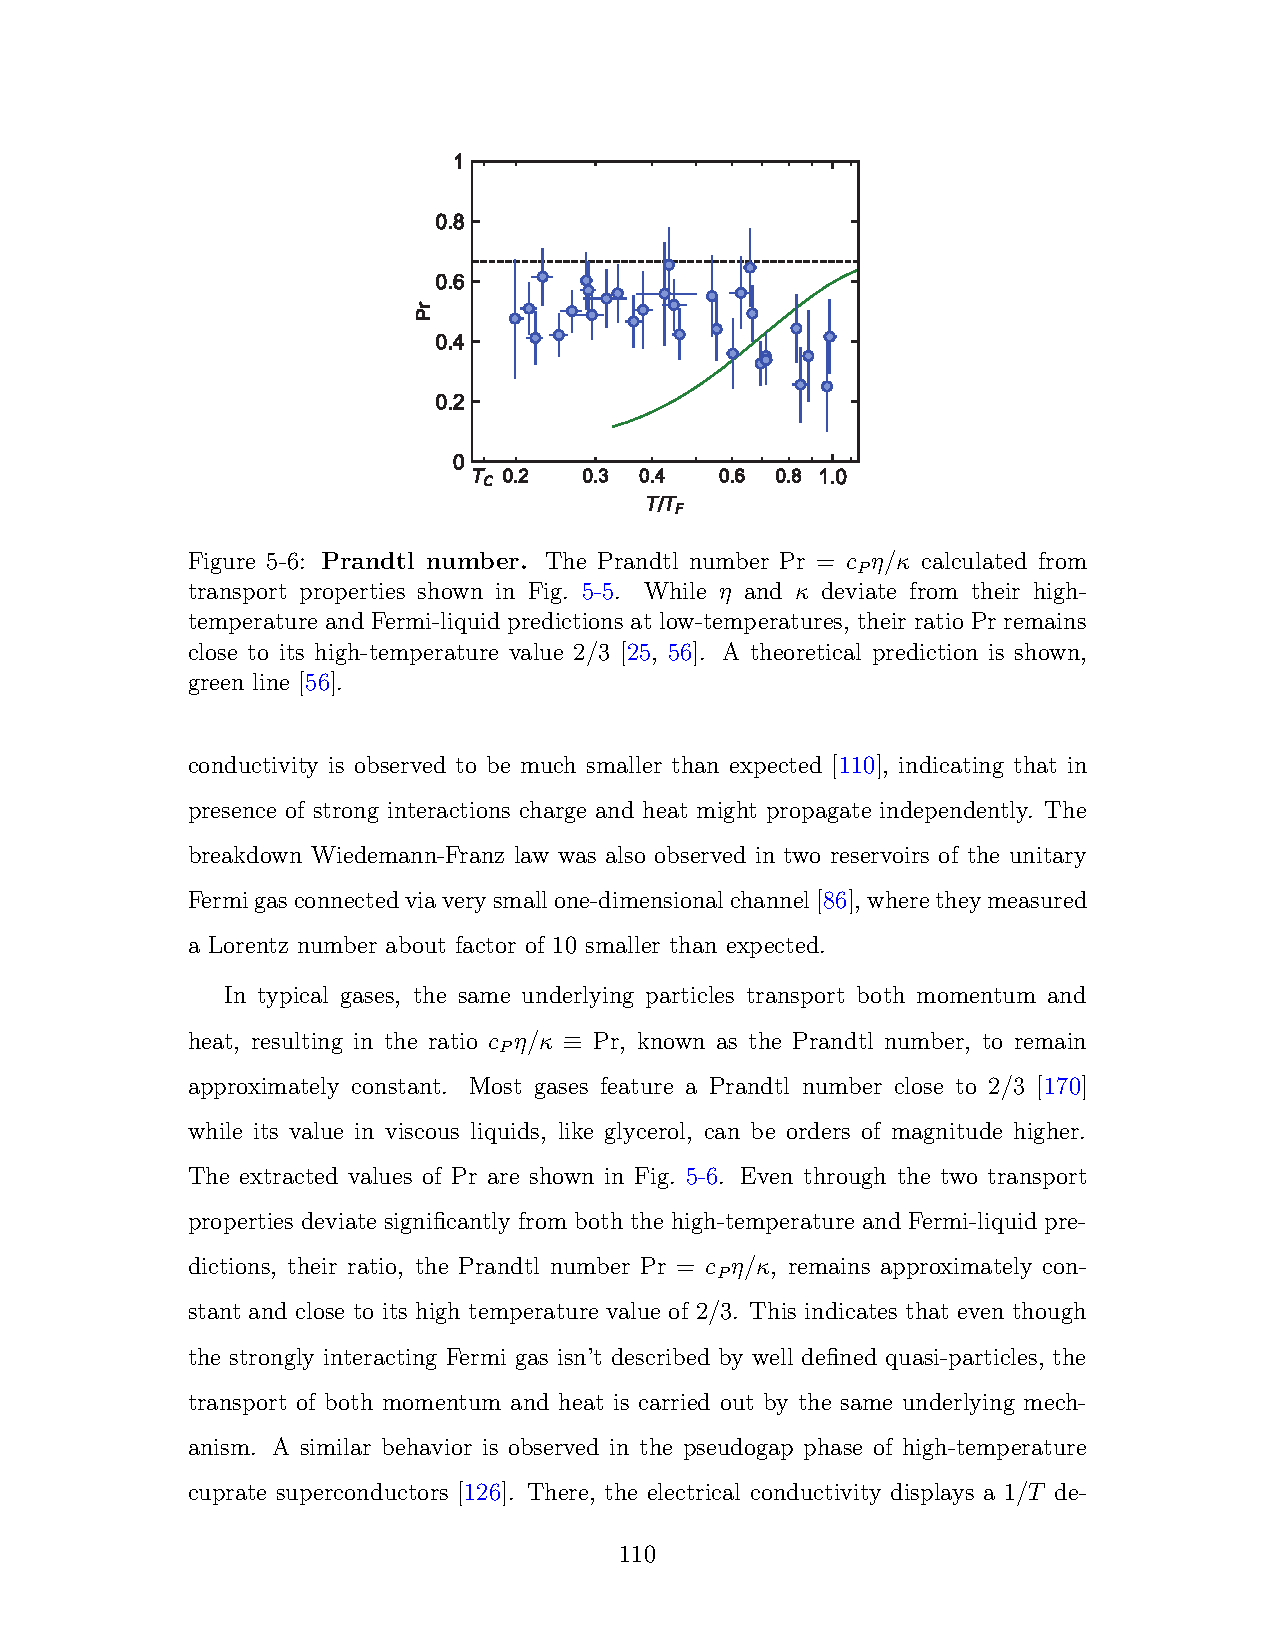
\includegraphics[width=0.9\textwidth,
		trim=7cm 19cm 7cm 2cm, clip]{figures/prandtl.pdf}
	\end{minipage}

	\vspace{-0.9cm}
	\begin{center}
		\begin{minipage}{0.4\textwidth}
			\mysmallerfont
			\centering 
			Red diamond [5], green line [6], pink line [7], cyan line [8], orange line [9] 
		\end{minipage}
	\end{center}
	
	}
	%\note[targetoffsetx=-16.5cm, targetoffsety=10cm, angle=0, radius=0cm,
	%width=0.8cm, rotate=0, connection, linewidth=0cm,
	%roundedcorners=0, innersep=0cm]{}

	%\note[targetoffsetx=0.3cm, targetoffsety=10cm, angle=0, radius=0cm,
	%width=0.9cm, rotate=0, connection, linewidth=0cm,
	%roundedcorners=0, innersep=0cm]{}
	
	
	
\end{columns}



\begin{columns} 
	\column{0.5}
	\colorlet{blocktitlebgcolor}{BEC1grey}
	\block[]{\textcolor{BEC1blue}{References}}
	{
	\begin{minipage}{0.2\textwidth}
		\myfont
		{[1]} B. Mukherjee et al., \textit{PRL} 2017\\
		{[2]} P.B. Patel et al., \textit{Science} 2020\\
		{[3]} Z. Yan et al., in preparation\\
		{[4]} M.J.H. Ku et al., \textit{Science} 2012
	\end{minipage}
	\begin{minipage}{0.2\textwidth}
		\myfont
		{[5]} L. Baird et al., \textit{PRL} 2019\\
		{[6]} B. Frank et al.,\textit{ Phys Rev Research} 2020\\
		{[7]} J. A. Joseph et al., \textit{PRL} 2015\\
		{[8]} M. Bluhm et al., \textit{PRL} 2017\\
		{[9]} T. Enss et al., \textit{Annals of Physics} 2011
	\end{minipage}


	} 
	
	
	\column{0.5} 
	\colorlet{blocktitlebgcolor}{BEC1grey}
	\block[]{\textcolor{BEC1blue}{Funding}}{

	\begin{minipage}{0.24\textwidth}
	
\includegraphics[height=4.4cm]{Funding Logos/Air_Force_LogoAsset 16.png}
	\hspace{0.23cm}
	
\includegraphics[height=4.4cm]{Funding Logos/NSF_Logo.png}
	\hspace{0.23cm}
	
\includegraphics[height=4.4cm]{Funding Logos/Office_of_Naval_Research_Official_Logo.png}
	\end{minipage}
	\hspace{1.5cm}
	\begin{minipage}{0.19\textwidth}
	\myfont
	\flushleft
	AFOSR-MURI, National Science Foundation, Office of Naval Research, Vannevar Bush Faculty Fellowship
	\end{minipage}
	\vspace{0.29cm}
}
	
	
	

	
\end{columns}





\end{document}